\section{Api de animación}
\subsection{Investigacion y conceptualización}
Después de imaginar y delimitar  y el problema a tratar, cómo primera instancia, se comenzó con la selección del tipo de entorno de trabajo que sería utilizado para el desarrollo del aplicativo ejecutable de manera local en la vivienda del solar decathlon, durante el transcurso del documento este programa será llamado "House Manager".
\vspace{0.5cm}\\
Para seleccionar el entorno de trabajo se realizó una averiguación de los posibles entornos de desarrollo que permitieran implementar programación orientada a objetos en dispositivos embebidos, dentro de los entornos de desarrollo más conocidos se observo; python, Java, procesing, c++, entre otros. Todos los anteriores con comunidades muy enfocada a su flexibilidad y constante mejoramiento.
\vspace{0.5cm}\\
Después se compararon a grandes rasgos los módulos de interfaz gráfica que ofrecían los entornos de programación mas conocidos y utilizados en la actualidad, como se puede observar a continuación:
\begin{itemize}
	\item En el caso de c++ se observo que el entorno de trabajo mas apropiado para desarrollar aplicativos gráficos era .net, la desventaja de este aplicativo era su estrecha relación con el lenguaje de programación de bajo nivel c\#, por ende el manejo de memoria del programa incrementba en gran medida los costos de desarrollo.
	
	\item Para Python se observo que los entornos de desarrollo de interfaz gráfica nativos tenían apariencias precarias similar a la nativa de windows 98, en adición, los frameworks mas estéticos tenían un soporte independiente al del lenguaje de programación como tal, por otra parte el lenguaje de programación como tal era multiplataforma y de muy alto nivel, lo que le permitiria al programador desarrollar algoritmos de mayor funcionalidad con menos lineas de código.
	
	\item En el caso de Java se observo que el entorno de desarrollo para interfaces gráficas era nativo del lenguaje de programación y permitía una mayor flexibilidad a la hora de desarrollar esquemas complejos con la exepción que se debía codificar detalladamente el comportamiento del objeto, lo que significaba mas tiempo de trabajo para el programador y archivos con mas lineas de codigo.
\end{itemize}

Como etapa de conceptualizacion, se realizo una primera version el diseño del aplicativo principal junto con sus respectivas escenas. Fig \ref{fig_0}. Los elementos utilizados en esta primera etapa de diseño se consistieron principalmente de: botones, caja de opciones, contenedores, y paneles animados. Para esta etapa de conceptualzacion no se tenia una paleta de colores escogida pero si se buscaba tener en cuenta tonalidades verdes siendo congruentes con la tematica amigable con el medio ambiente que rodea al Solar Decathlon, tambien, se persiguio el poder seleccionar a partir de la pantalla principal diferentes "sub aplicativos" que podrian ser diseñados de manera independiente.

\begin{figure}[htbp]
	\centerline{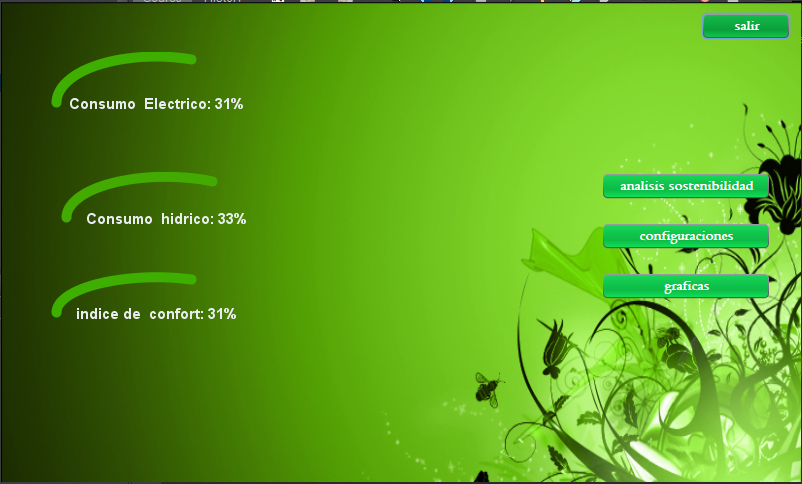
\includegraphics[width=8.5cm]{figuras/houseManager1.png}}
	\caption{Conceptualización inicial de la api en sitio}
	\label{fig_0}
\end{figure}

Para hacer realidad el diseño de esta primera etapa de conceptualizacion se utilizo como lenguaje de programacion el lenguaje de programación Java puesto que representaba en su mayor parte el lenguaje más utilizado en la Universidad del Valle durante el momento.

\begin{figure}[htbp]
	\centerline{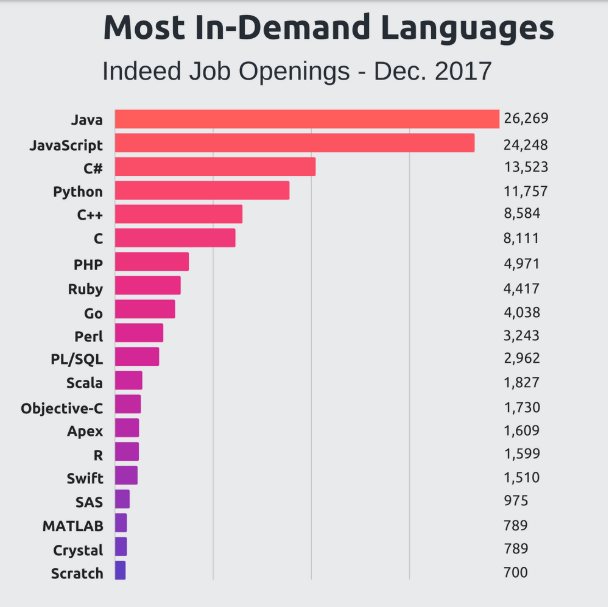
\includegraphics[width=8.5cm]{./figuras/stadistics_job.png}}
	\caption{Estadisticas de los lenguajes de programacion con más demanda}
	\label{fig_1}
\end{figure}

En adición, Java es un lenguaje de programacion de muy alta demanda, de hecho, el de mayor ofertas de trabajo registradas durante el 2017 en el portal de trabajo internacional \href{https://co.indeed.com/?r=us}{indeed.com}, seguido de javascript, c\# y python, tal como se observa en la figura \ref{fig_1}.

\subsection{Api de java}
Todos los objetos implementados para esta api fueron desarrollados estrictamente con java puro y sin librerias externas con el objetivo de obtener un codigo limpio, totalmente multiplataforma y que heredara paquetes unicamente de los modulos swing nativos de java. Como primera instancia se desarrollo el componente funcional de la API, es decir la parte programática, y finalmente se escribió el javadoc, el cual es un documento integrado que describe como se deben usar los objetos 
\vspace{0.5cm}\\
Normalmente para java es necesario construir y empaquetar el codigo que contenga la interaccion de manera manual con java puro. Por ejemplo, en javascript es posible enlazar funciones directamente sin acceder a paquetes adicionales como los "event listeners" de java, puesto que todo es considerado un objeto; desde un numero hasta una funcion.	
\vspace{0.5cm}\\
El primer objeto desarrollado en la api de java fue el boton personalizado, usando este objeto contenido en la api se puede crear un boton de cualquier tamaño con una, dos o tres imagenes para los estados; "normal", "presionado" y "encima". Un ejemplo de la utlizacion de la api se puede ver en la figura \ref{fig_2}. este objeto funciona ajustando automaticamente su tamaño basado en la resolución de las imagenes, esto para complementar con una metodologia de diseño: primero el dibujo, luego el programa.

\begin{figure}[htbp]
	\centerline{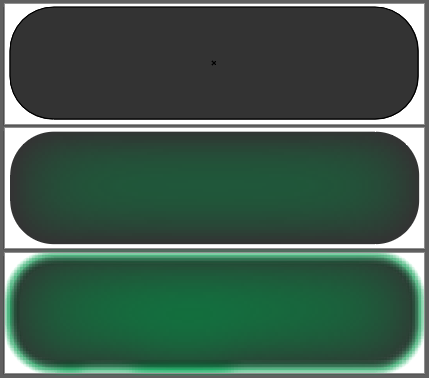
\includegraphics[width=8.5cm]{./figuras/boton.png}}
	\caption{El diseño de estados del boton interactivo}
	\label{fig_2}
\end{figure}

El segundo objeto grafico desarrollado fue un boton expandible o "caja de opciones", que permitiera generar un boton desplegable con la posibilidad de modificar texto de manera superficial basado en dos o tres imagenes para la parte superior, inferior y media respectivamente. Un implementacion utlizada en la aplicacion se puede observar en la figura \ref{fig_3}. cada una de las imagenes del boton desplegable debe tener sus 3 imagenes de estado: normal, presionado y encima para interactuar de manera dinamica con el mouse.

\begin{figure}[htbp]
	\centerline{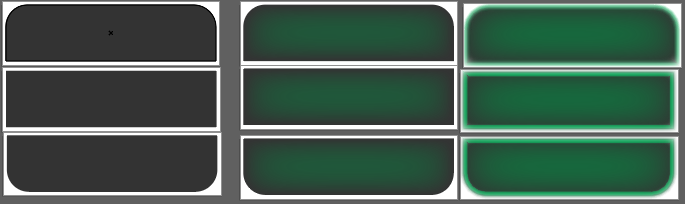
\includegraphics[width=7.5cm]{./figuras/boton_desplegable.png}}
	\caption{El diseño de los estados del boton interactivo desplegable}
	\label{fig_3}
\end{figure}

Como tercer objeto grafico, se desarrollo un objeto de animacion que podia mover un objeto tipo swing (esta es la clase madre de la mayoria de los objetos graficos en java) en 4 posibles direcciones; las dos horizontales y las dos verticales, tal como se observa en la figura \ref{fig_4}. La funcion permite modificar la ubicacion actual del objeto moviendolo de manera linear con una rata de refresco dada (actualizacion visual) y una velocidad constante, desde una cordenada X o Y dependiendo de en cual eje coordenado se desee mover el componente.

\begin{figure}[htbp]
	\centerline{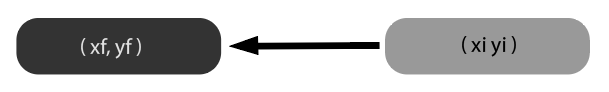
\includegraphics[width=7.5cm]{./figuras/boton_movimiento.png}}
	\caption{Movimiento según la ubicación de la función horizontal}
	\label{fig_4}
\end{figure}

El desarrollo de la api fue de importancia para la construccion de la primera version del aplicativo en sitio, la primera version se puede observar en la figura \ref{fig_5}, debido a la recursiva implementacion grafica se obtuvo un programa que sobrecargaba un sistema de computo completo (portatil dell con procesador i5 segunda generacion, 4gb de ram DDR3, y un disco duro HDD). Por lo tanto se busco cambiar el entorno de desarrollo a uno con mas flexibilidad a la hora del diseño grafico, con capacidad de funcionar en sistemas de más bajo computo tipo Single Computer Boards como la Raspberry o la Beaglebone. Para probar el desempeño de la api, se realizaron pruebas con los elementos ya diseñados en la api de Java y se observo que resultaba una carga para el cpu realizar las animaciones, principalmente, cuando se deseaba mover más de 5 objetos Jswing.

\begin{figure}[htbp]
	\centerline{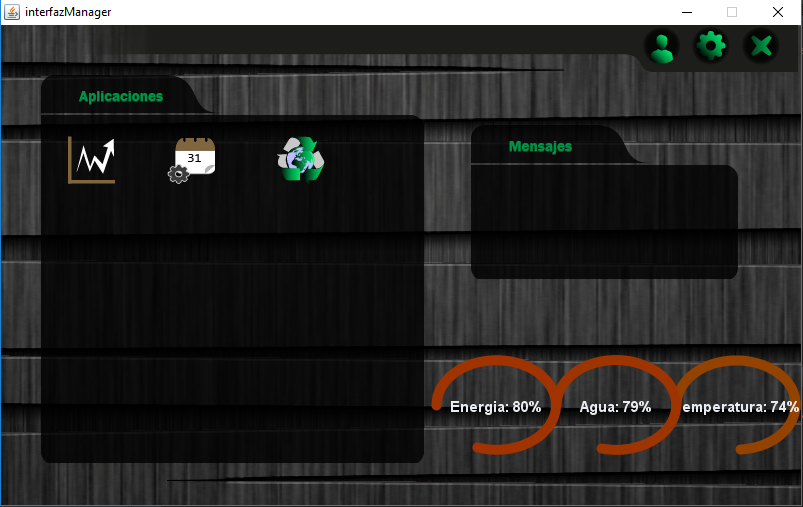
\includegraphics[width=8.5cm]{./figuras/houseManager23.png}}
	\caption{Primer Approximación del diseño de la interfáz en sitio}
	\label{fig_5}
\end{figure}

Despues de haber programado los elementos necesarios para generar la estructura basica del aplicativo se replanteo el diseño con una estructura más moderna y parecidas a las tendencias en diseño movil tal como se observa en la figura \ref{fig_21} con el objetivo de que se percibiera que ambos aplicativos dearrollados en este sistema podian ofrecer los mismos servicios. Ademas, generar una experiencia de usuario similar en ambas plataformas

\begin{figure}[htbp]
	\centerline{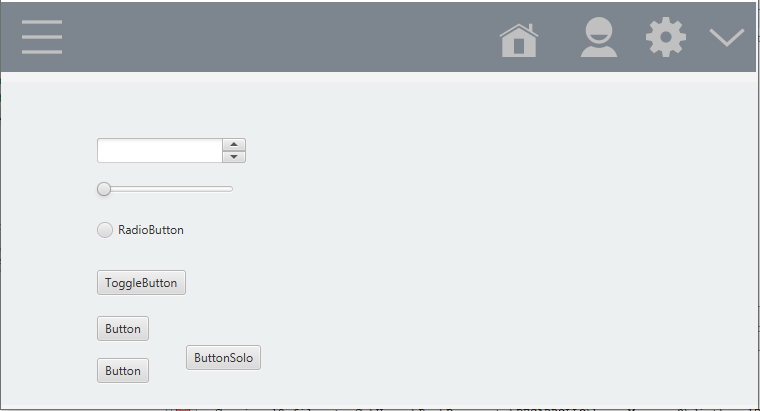
\includegraphics[width=8.5cm]{./figuras/house_manager_version_2.png}}
	\caption{Ajuste de diseño de la interfáz en sitio}
	\label{fig_21}
\end{figure}

En un tercer nivel de conceptualizacion se re diseño la interfaz grafica estandarizando y simplificando los componentes que esta contenia; se selecciono la paleta de colores y agregaron algunos nuevos objetos al diseño generalizado como se puede observar en la figura vease en la figura \ref{fig_22}. Para la correcta seleccion de la paleta de colores se busco generar una simetria triangular en el espacio de colores HSV, usando como referencia un color sacado del logo oficial de la "Chameleon house" (nombre oficial de la casa diseñada para el solar decathlon). 

\begin{figure}[htbp]
	\centerline{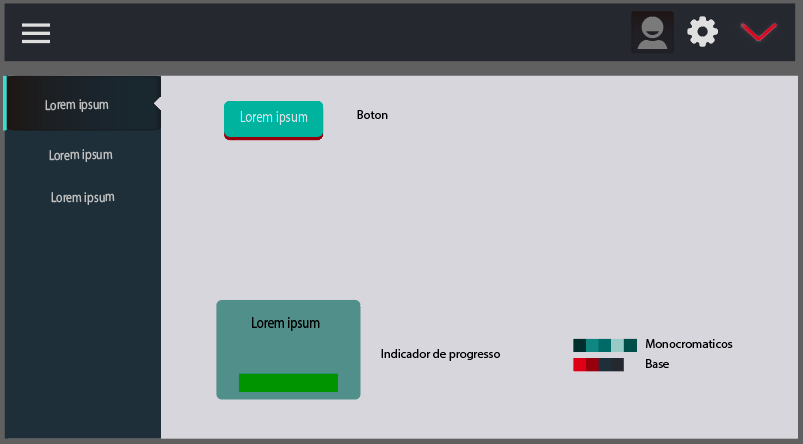
\includegraphics[width=8.5cm]{./figuras/house_manager_version_3.png}}
	\caption{Version final del concepto de diseño}
	\label{fig_22}
\end{figure}

Debido a la estructura de Java, codificar todos los nuevos objetos resultaba una tarea de mayor trabajo y con baja recompensa, es decir, mas lineas de codigo por objeto; como sólucion se traducio lo que se tenia desarrollado hasta el momento de la api a un lenguaje de programacion de mas alto nivel (Python) y se utilizo un framework exclusivamente para el desarrollo de la interfaz grafica, debido a que se trataba de un modulo completamente estrito en C le permitia a la aplicacion tener un mejor rendimiento grafico, con la desventaja de dificultar el efecto multiplataforma de python, para mantener el efecto, el framework deberia soportar por completo la plataforma sobre la cual se estuviera corriendo (Windows, mac'os, linux, ubuntu, etc).

\subsection{Api de Python y Qt}

El framework utilizado para desarrollar los modulos graficos se llama Qt y para poder utilizarlo es necesario instalar unas dependencias C especificas y la lipreria respectiva para Python. Una vez Qt esta correctamente configurado el diseño estatico del aplicativo se realiza a partir de un "lenguaje de marcado" (markup language) autogenerado llamado Qml que define las propiedades graficas estáticas de los objetos a utilizar, el Qml viene de la mano con un lenguaje tipo "hoja de estilo" (style sheet), a partir del cual se le adjudican propiedades interactivas y estilos que en conjunto son comprendidos por python y su libreria Pyside.
Para esta etapa de diseño se utilizó una paleta de colores complementarios para los objetos importantes y tonalidades oscuras de grises azulados para los fondos. Todos dentro del espectro de colores de la marca de la casa del Solar Decathlon Latinoamerica de la Universidad del Valle  


Teniendo en cuenta el nuevo framework se utilizo la herramienta de diseño de Qt desing (oficial del framework) para codificar de manera automatica las propiedades estaticas de la interfaz grafica. Tambien, se codificaron manualmente las propiedades dinamicas en un archivo de Qss que luego fue cargado por la libreria Pyside para ser procesado como un objeto Python. 
\vspace{0.5cm}\\
Primero, se codifico un boton de la misma manera como se codifico el codigo de la API para Java; con este opjeto de python se puede crear un boton de cualquier tamaño con una, dos o tres imagenes para los estados; "normal", "presionado" y "encima". Un ejemplo de la utlizacion de la api se puede ver en la figura \ref{fig_19}.

\begin{figure}[htbp]
	\centerline{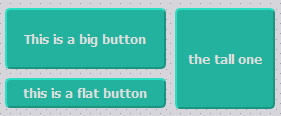
\includegraphics[width=7.5cm]{./figuras/qt_button.png}}
	\caption{Botón de tamaño flexible genérico de la api de qt}
	\label{fig_19}
\end{figure}

segundo se codifico un boton generico con las mismas funcionalidades del boton anterior, pero en lugar de funcionar basado en imagenes funcionaba con un color dado y las interacciones "normal", "presionado" y "encima" son calcuadas atenuando y resaltando el color para generar un efecto de sombra e iluminacion. Para el aplicativo se utilizo el color mostrado en la figura \ref{fig_20}.


Tercero, se desarrollo un expandible o "caja de opciones", personalizada, para ello se modifico el objeto qss Qoptionbar que permite generar un boton desplegable con la posibilidad de modificar texto de manera superficial basado en un color especifico.

Cuarto, se programo una barra deslizable para facilitar el proceso de ingresar datos numericos a la aplicacion desde una interfa tactil. Nuevamente se usaron los colores de la paleta de colores seleccionada y se opto por la solucion de diseño mas sencilla posible tal como se puede ver en la imagen \ref{fig_20}

\begin{figure}[htbp]
	\centerline{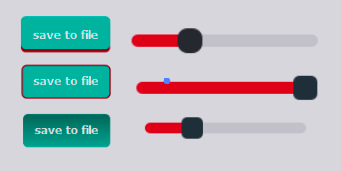
\includegraphics[width=7.5cm]{./figuras/qt_button_slide.png}}
	\caption{Boton de tamaño fijo usando imagenes y slider}
	\label{fig_20}
\end{figure}

Finalmente se personalizaron los colores de todos los espacios y elementos secundarios utilizados, como: la grafica, la barra de menu, los botones especiales del menu, etc.







